\documentclass[a4paper,11pt,oneside]{article}

\usepackage[utf8]{inputenc}
\usepackage[T1]{fontenc}
\usepackage[english]{babel}
\usepackage{amssymb}
\usepackage{amsmath}
\usepackage{amsthm}
\usepackage{graphicx}
\usepackage{float}
\usepackage{hyperref}
\usepackage[dvipsnames]{xcolor}
\usepackage{tcolorbox}
\usepackage[top=2cm, bottom=2.5cm, right=2.5cm, left=2.5cm]{geometry}

\newtheorem{theorem}{Theorem}
\theoremstyle{definition}
\newtheorem{definition}{Definition}
\hypersetup{colorlinks=true,urlcolor=blue,linkcolor=blue}
\renewcommand{\familydefault}{\sfdefault}
\parindent0pt
\parskip6pt

\begin{document}

\title{Proof of the Erlang C formula}
\author{Alexander Herzog\\\href{mailto:alexander.herzog@tu-clausthal.de}{\small\texttt{alexander.herzog@tu-clausthal.de}}\\\href{https://a-herzog.github.io/QueueCalc/}{\small\texttt{a-herzog.github.io/QueueCalc}}}
\date{}

\maketitle



\section{The Erlang C model}

The Erlang C queueing model describes a service system with exponentially distributed inter-arrival times with an arrival rate of $\lambda>0$, exponentially distributed service times with a service rate of $\mu>0$ and $c\in\mathbb{N}$ operators at the service desk. The arriving customers form a queue in front of the service desk. Each time an operator gets idle, the customer who has waited for the longest time will be routed to the free operator (FIFO queueing discipline; first-in-first-out), see figure \ref{fig:Model}.

\begin{figure}[H]
\begin{center}
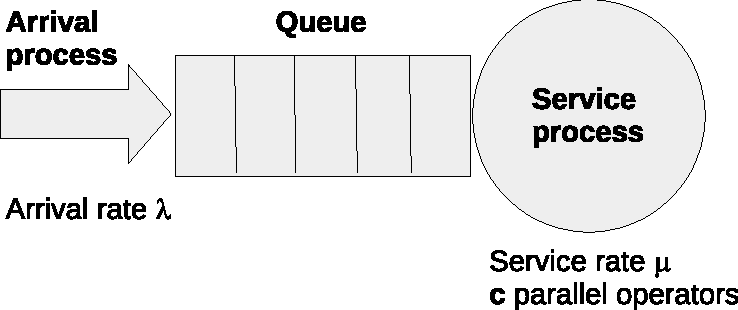
\includegraphics[width=0.6\textwidth]{ProofOfTheErlangCFormula-Model.pdf}
\end{center}
\caption{Erlang C queueing model}
\label{fig:Model}
\end{figure}

The long-run utilization of the system is
$$
\rho:=\frac{\lambda}{c\mu}\;.
$$
The system can only operate stably in the long term if $\rho<1$ (the long-run arrival rate is lower than the available workforce).

The following indicators are usually of interest:
\begin{itemize}
\item
$P(W\le t)$: probability for a new arriving customer to have to wait no longer than $t\ge0$ seconds (Erlang C formula),
\item
$\mathbf{E}[W]$: average waiting time,
\item
$\mathbf{E}[V]$: average residence time,
\item
$\mathbf{E}[N_Q]$: average number of customers in the queue,
\item
$\mathbf{E}[N]$: average number of customers in the system.
\end{itemize}



\section[Idea for calculating P(W<=t)]{Idea for calculating $P(W\le t)$}

The idea for calculating the customer's waiting time distribution $P(W\le t)$ (the probability that the customer has to wait at most $t\ge0$ seconds) is to determine the waiting time probability distribution for all possible states in which the system can be and to weight these times with the probability that the system is in the respective state. This leads to the formula:
\begin{equation}\label{eq:WaitingTimeDistribution1}
P(W\le t)=\sum_{n=0}^\infty P_{\mu,n-(c-1)}(W\le t)\cdot p_n
\end{equation}
where $p_n$ in the probability that there are $n$ customers in the system and $P_{\mu,m}(W\le t)$ is the probability for a new customer to have to wait $t$ or less seconds in the case the service rate is $\mu>0$ and there are $m$ customers that will have to be served to the end before the new customer's service process starts. For $m=0$ the new service process will start immediately ($P_{\mu,0}(W\le t)=1$ for all $t\ge0$) and for consistence we assume the same for $m<0$.

\paragraph{Case $n\ge c$:}~\\
If there are $n<c$ customers in the system, a newly arriving customer can be served immediately, as in this case not all operators are currently busy. If $n\ge c$, one or more already running service processes has to end first, and then any customers who were already waiting before the newly arrived customer must be served before the newly arrived customer can be served. A distinction must therefore be made between the service times of customers whose service has yet to begin and the remaining service times of customers who are already in the service process. However, since the Erlang models uses the exponential distribution for the service times, these two time durations are subject to the same probability distribution with the same parameter. This is due to the memorylessness of the exponential distribution. (This property of the exponential distribution will be proofed below in section \ref{ExponentialDistribution}).

\paragraph{Case $n<c$:}~\\
For $n<c$ customers in the system, the probability that a newly arriving customer will have to wait less than $t\ge0$ seconds is always 1 for all $t\ge0$ (the newly arriving customer does not have to wait at all). This means we have $P_{\mu,n-(c-1)}(W\le t)=1$ for $n<c$ and for all $t\ge0$ and formula \eqref{eq:WaitingTimeDistribution1} can be simplified to:
\begin{equation}\label{eq:WaitingTimeDistribution2}
P(W\le t)=\sum_{n=0}^{c-1} p_n+\sum_{n=c}^\infty P_{\mu,n-(c-1)}(W\le t)\cdot p_n\;.
\end{equation}

Since $P_{\mu,n-(c-1)} (W\le t)$ represents the sequential execution of several exponential distributions (and thus is an Erlang distribution, see section \ref{ErlangDistribution}) and $p_n$ is the probability that the corresponding Markov chain is in state $n$, the following sections will present results on exponential distributions (section \ref{ExponentialDistribution}), Erlang distributions (section \ref{ErlangDistribution}), and birth-and-death processes (section \ref{BirthAndDeathProcesses}), which will ultimately allow us to calculate formula \eqref{eq:WaitingTimeDistribution2} in section \ref{Result}.



\section{Exponential distribution}\label{ExponentialDistribution}

Since the inter-arrival and the service times are distributed due to the exponential distribution in an Erlang model, we will need some results for the exponential distribution which will be presented and proofed here.

\begin{definition}[Probability density function of the exponential distribution]
The function
$$
f_{\lambda}(x):=\left\{\begin{matrix}
\lambda \mathrm{e}^{-\lambda x},&~x\ge0\;,\\
0,&~x<0
\end{matrix}\right.
$$
with $\lambda>0$ is called the probability density function of the exponential distribution.
\end{definition}

\begin{theorem}[Cumulative distribution function of the exponential distribution]
The function
$$
F_{\lambda}(x):=\left\{\begin{matrix}
1-\mathrm{e}^{-\lambda x},&~x\ge0\;,\\
0,&~x<0
\end{matrix}\right.
$$
is the cumulative distribution function of the exponential distribution with probability density function $f_\lambda(x)$, $\lambda>0$.
\end{theorem}

\begin{proof}
According to the definition of the cumulative distribution function $F(x):=\int_{-\infty}^x f(t)\,\mbox{d}t$ holds:
$$
F_\lambda(x)=\int_0^x \lambda \mathrm{e}^{-\lambda t}\,\mbox{d}t=\left[-\mathrm{e}^{-\lambda t}\right]_{t=0}^{t=x}=-\mathrm{e}^{-\lambda x}-(-1)=1-\mathrm{e}^{-\lambda x}
$$
for $x\ge0$ and $F_\lambda(x)=0$ else.
\end{proof}

\begin{theorem}
The function $f_\lambda(x)$, $\lambda>0$, is the probability density function of a probability distribution, i.\,e.\ $f_\lambda(x)\ge0$ and $\int_{-\infty}^\infty f_\lambda(x)\,\mbox{d}x=1$.
\end{theorem}

\begin{proof}
The proposition $f_\lambda(x)\ge0$ follows directly from the definition of $f_\lambda(x)$. The previous theorem gives us:
$$
\int_{-\infty}^\infty f_\lambda(t)\,\mbox{d}t=\lim_{x\to\infty}F_\lambda(x)=\lim_{x\to\infty}1-\mathrm{e}^{-\lambda x}=1\;.
$$
\end{proof}

\begin{theorem}[Indicators of the exponential distribution]
For an exponential distribution with parameter $\lambda>0$, the following holds:
\begin{enumerate}
\item $\mathbf{E}[X]=\frac{1}{\lambda}$,
\item $\mathbf{Std}[X]=\frac{1}{\lambda}$ and
\item $\mathbf{CV}[X]=\mathbf{SCV}[X]=1$.
\end{enumerate}
\end{theorem}

\begin{proof}
\begin{enumerate}
\item
With the definition of $\mathbf{E}[X]$ follows:
\begin{eqnarray*}
\mathbf{E}[X]&=&
\int_{-\infty}^\infty x\cdot f_\lambda(x)\,\mbox{d}x=
\int_0^\infty \lambda x \mathrm{e}^{-\lambda x}\,\mbox{d}x\\&=&
\left[\lambda x\cdot\left(-\frac{1}{\lambda}\right)\mathrm{e}^{-\lambda x}\right]_{x=0}^{x=\infty}-
\int_0^\infty \lambda \left(-\frac{1}{\lambda}\right)\mathrm{e}^{-\lambda x}\,\mbox{d}x=
0+\int_0^\infty\mathrm{e}^{-\lambda x}\,\mbox{d}x\\&=&
\left[\left(-\frac{1}{\lambda}\right)\mathrm{e}^{-\lambda x}\right]_{x=0}^{x=\infty}=
0-\left(-\frac{1}{\lambda}\right)=
\frac{1}{\lambda}\;.
\end{eqnarray*}
\item
With the definition of $\mathbf{E}[X^2]$ follows initially:
\begin{eqnarray*}
\mathbf{E}[X^2]&=&
\int_{-\infty}^\infty x^2\cdot f_\lambda(x)\,\mbox{d}x=
\int_0^\infty \lambda x^2 \mathrm{e}^{-\lambda x}\,\mbox{d}x\\&=&
\left[\lambda x^2 \left(-\frac{1}{\lambda}\right)\mathrm{e}^{-\lambda x}\right]_{x=0}^{x=\infty}-
\int_0^\infty 2\lambda x \left(-\frac{1}{\lambda}\right)\mathrm{e}^{-\lambda x}\,\mbox{d}x=
0+\int_0^\infty 2x\mathrm{e}^{-\lambda x}\,\mbox{d}x\\&=&
\left[2x \left(-\frac{1}{\lambda}\right)\mathrm{e}^{-\lambda x}\right]_{x=0}^{x=\infty}-
\int_0^\infty 2\left(-\frac{1}{\lambda}\right)\mathrm{e}^{-\lambda x}\,\mbox{d}x=
0+\frac{2}{\lambda}\left[\left(-\frac{1}{\lambda}\right)\mathrm{e}^{-\lambda x}\right]_{x=0}^{x=\infty}\\&=&
0-\frac{2}{\lambda}\left(-\frac{1}{\lambda}\right)=
\frac{2}{\lambda^2}\;.
\end{eqnarray*}
Using the shift theorem we get:
$$
\mathbf{Var}[X]=\mathbf{E}[X^2]-\left(\mathbf{E}[X]\right)^2=\frac{2}{\lambda^2}-\left(\frac{1}{\lambda}\right)^2=\frac{1}{\lambda^2}\;.
$$
And so, ultimately, the following applies to the standard deviation:
$$
\mathbf{Std}[X]=\sqrt{\mathbf{Var}[X]}=\frac{1}{\lambda}\,.
$$
\item
From 1 and 2 follows directly:
$$
\mathbf{CV}[X]=\frac{\mathbf{Std}[X]}{|\mathbf{E}[X]|}=\frac{\frac{1}{\lambda}}{\frac{1}{\lambda}}=1\,.
$$
Furthermore, $\mathbf{SCV}[X]=\left(\mathbf{CV}[X]\right)^2=1$.
\end{enumerate}
\end{proof}

\subsection{Memorylessness of the exponential distribution}

\begin{theorem}[Memorylessness of the exponential distribution]
If a time interval is exponentially distributed and the event has not yet occurred at time $s\ge0$, then the time distribution that the event will occur within the next $t\ge0$ time units (i.\,e.\ up to time $s+t$), is again exponentially distributed with the same parameter $\lambda>0$, i.\,e.\ the following applies:
\begin{equation}\label{eq:DefinitionMemorylessness}
P(X\le t+s | X\ge s)=P(X\le t)\;,
\end{equation}
where $P(X\le a| X\ge b)$ is the conditional probability of the event "$X\le a$" knowing in advance that $X\ge b$.
\end{theorem}

\begin{proof}
Using the calculation rules for conditional probabilities, the following holds:
\begin{eqnarray*}
P(X\le t+s | X\ge s)&=&
\frac{P(\{X\le t+s\}\cap\{X\ge s\})}{P(X\ge s)}=
\frac{F_\lambda(t+s)-F_\lambda(s)}{1-F_\lambda(s)}\\&=&
\frac{1-\mathrm{e}^{-\lambda(t+s)}-1+\mathrm{e}^{-\lambda s}}{1-(1-\mathrm{e}^{-\lambda s})}=
\frac{\mathrm{e}^{-\lambda s}-\mathrm{e}^{-\lambda(t+s)}}{\mathrm{e}^{-\lambda s}}=
1-\mathrm{e}^{-\lambda t}\\&=&
F_\lambda(t)=
P(X\le t)\;.
\end{eqnarray*}
\end{proof}

\paragraph{Consequence:}~\\
If the service time of a customer is exponentially distributed with parameter $\lambda>0$ and the customer is already in the service process, then the remaining service time of the customer is again exponentially distributed with the same parameter $\lambda$. If the cumulative distribution function of the waiting time of a newly arriving customer is to be determined, no distinction needs to be made between the remaining service times of the customers currently being served and the service times of the other customers waiting before the newly arrived customer.

\begin{theorem}
The exponential distribution $F_\lambda(x)$ is the only \emph{continuous} probability distribution with $F(x)=0$ for $x\le0$ that has the property of memorylessness.
\end{theorem}

\begin{proof}
The proof consists of three steps:

\paragraph{Step 1: Functional equation describing the memorylessness}~\\
In order to present the proof as simply as possible, we first define the function $G(t):=1-F(t)$, which indicates the probability that the event has \emph{not yet} occurred by time $t\ge0$. (This definition comes from reliability theory, where $G(t)$ is called the \emph{survival probability}.) From equation \eqref{eq:DefinitionMemorylessness}, using the calculation rules for conditional probabilities, we get:
\begin{eqnarray*}
~&~&P(X\le t+s | X\ge s)=P(X\le t)
~\iff~\frac{F(t+s)-F(s)}{1-F(s)}=F(t)\\
~&\iff&\frac{1-G(t+s)-(1-G(s))}{G(s)}=1-G(t)\\
~&\iff&-G(t+s)+G(s)=G(s)-G(s)G(t)
~\iff~G(s+t)=G(s)G(t)\,.
\end{eqnarray*}
Therefore, we have to show that only the survival probability assuming an exponential distribution, i.e., $G_\lambda(t)=\mathrm{e}^{-\lambda t}$, satisfies the equation $G(s+t)=G(s)G(t)$.

\paragraph{Step 2: Explicit representation for $G(t)$}~\\
From $G(s+t)=G(s)G(t)$ follows for $a\in\mathbb{N}$ and $b\in\mathbb{N}$:
\begin{eqnarray*}
G\left(\frac{a}{b}\right)&=&
G\left(\frac{1}{b}+\frac{a-1}{b}\right)=
G\left(\frac{1}{b}\right)\cdot G\left(\frac{a-1}{b}\right)=
\ldots=
\underbrace{G\left(\frac{1}{b}\right)\cdots G\left(\frac{1}{b}\right)}_{a~\textrm{factors}}\\
~&=&\left[G\left(\frac{1}{b}\right)\right]^a\,.
\end{eqnarray*}
From $1=\frac{b}{b}$ follows $G(1)=\left[G\left(\frac{1}{b}\right)\right]^b$ respectively $\left[G(1)\right]^{\frac{1}{b}}=G\left(\frac{1}{b}\right)$.
This leads to:
$$
G\left(\frac{a}{b}\right)=
\left[G\left(\frac{1}{b}\right)\right]^a=
\left[G(1)\right]^{\frac{a}{b}}\,.
$$
This means that the relationship $G(q)=[G(1)]^q$ holds for all positive rational numbers $q$. Due to the fact that $F$ was assumed to be continuous and therefore $G$ is also continuous, $G(t)=[G(1)]^t$ applies for all real $t\ge0$. Furthermore, the following applies with the calculation rules for the exponential and logarithms function:
$$
G(t)=
\mathrm{e}^{\ln\left(G(1)^t\right)}=
\mathrm{e}^{t\ln(G(1))}\,.
$$
Choosing $\lambda:=-\ln(G(1))$ yields $G(t)=\mathrm{e}^{-\lambda t}$ and $F(t)=1-\mathrm{e}^{-\lambda t}$.
It remains to be shown that $0<\lambda<\infty$ respectively $0<G(1)<1$ applies.

\paragraph{Step 3: Proof that $0<G(1)<1$ holds}~\\
It was $G(1)=1-F(1)$. This immediately implies that $0\le G(1)\le1$. It remains to show that $0\neq G(1)\neq1$.
\begin{itemize}
\item
If $G(1)=0$, then $G(x)=\left[G(1)\right]^x=0^x=0$ would apply for all $x>0$. This would mean that $F(x)=1$ for all $x>0$. However, since $F$ was assumed to be continuous and $F(0)=0$ according to the assumption, this cannot be the case.
\item
If $G(1)=1$, then $G(x)=\left[G(1)\right]^x=1^x=1$ would hold for all $x\ge0$. This would mean that $F(x)=0$ for all $x\ge0$, which contradicts the fact that $F(x)$ is the cumulative distribution function of a probability distribution and therefore $\lim_{x\to\infty}F(x)=1$ must hold.
\end{itemize}
\end{proof}



\section{Convolution of probability distributions}

If two processes that can be described by probability distributions are executed one after the other, we say that the probability density functions of the two probability distributions are convolved with each other. The result of the convolution is the probability density function of the probability distribution that describes the overall process.

\begin{definition}[Convolution]
If $f(x)$ and $g(x)$ are probability density functions of two probability distributions, the expression
$$
f*g(x):=\int_{-\infty}^\infty f(t)g(x-t)\,\mbox{d}t
$$
is called the convolution of $f$ and $g$.
\end{definition}

Illustratively, the above formula integrates all conceivable cases in which the total time $x$ can be divided between the two subprocesses $f$ and $g$.

Since convolution is defined by an integral over the product of two probability density functions, it is the case that for all probability distributions where it is difficult to determine the integral of the probability density functions -- which applies to almost all continuous probability distributions except the exponential distribution -- it is very difficult or impossible to calculate explicitly. This is the reason why the exponential distribution is always used for service times in the Erlang formulas.



\section{Erlang distribution}\label{ErlangDistribution}

As we will see next, the Erlang distribution describes a process consisting of the sequential execution of $n\in\mathbb{N}$ subprocesses, each of which has an exponential distribution with the same parameter $\lambda>0$.

In an M/M/1 system, the waiting time distribution of a newly arriving customer can be represented by the service times of the customers waiting in front of him and the remaining service time of the customer currently being served. However, due to the memorylessness of the exponential distribution (see equation \eqref{eq:DefinitionMemorylessness}), the remaining service time of the customer currently being served is distributed in the same way as his total service time. This means that if there are $k\ge0$ customers already waiting in the queue before the newly arriving customer and the service times are exponentially distributed with parameter $\mu\ge0$, then the waiting time of the new customer is Erlang distributed with parameters $\mu$ and $k+1$.

\begin{definition}[Probability density function of the Erlang distribution]
The function
$$
f_{\lambda,n}(x):=\left\{\begin{matrix}
\frac{\lambda^n x^{n-1}}{(n-1)!} \mathrm{e}^{-\lambda x},&~x\ge0\;,\\
0,&~x<0
\end{matrix}\right.
$$
with $\lambda>0$ and $n\in\mathbb{N}$ is called the probability density function of the Erlang distribution.
\end{definition}

\begin{theorem}[Connection to the exponential distribution]
The function $f_{\lambda,n}(x)$, $\lambda>0$, $n\in\mathbb{N}$ is the $n$-fold convolution of $f_\lambda(x)$.
\end{theorem}

\begin{proof}
The proof is carried out by induction. Obviously it is true that $f_{\lambda,1}(x)=\lambda \mathrm{e}^{-\lambda x}=f_\lambda(x)$. For the convolution of two exponentially distributed time durations, the following applies:
$$
f_{\lambda,1}*f_\lambda(x)=
f_\lambda*f_\lambda(x)=
\int_0^x \lambda \mathrm{e}^{-\lambda t}\cdot\lambda \mathrm{e}^{-\lambda(x-t)}\,\mbox{d}t=
\left[\lambda^2\mathrm{e}^{-\lambda x}t\right]_{t=0}^{t=x}=
\lambda^2x\mathrm{e}^{-\lambda x}=f_{\lambda,2}(x)
$$
for $x\ge0$ and $f_{\lambda,2}(x)=0$ else. Now we assume that
$$
f_{\lambda,n}(x)=\underbrace{f_\lambda*\cdots*f_\lambda}_{n~{\rm-times}}(x)
$$
for some $n\in\mathbb{N}$.
Then holds:
\begin{eqnarray*}
f_{\lambda,n}*f_\lambda(x)&=&
\int_0^x \frac{\lambda^n t^{n-1}}{(n-1)!}\mathrm{e}^{-\lambda t}\cdot\lambda \mathrm{e}^{-\lambda(x-t)}\,\mbox{d}t=
\frac{\lambda^{n+1}}{(n-1)!}\mathrm{e}^{-\lambda x}\int_0^x t^{n-1}\,\mbox{d}t\\&=&
\frac{\lambda^{n+1}}{(n-1)!}\mathrm{e}^{-\lambda x}\left[\frac{1}{n}t^n\right]_{t=0}^{t=x}=
\frac{\lambda^{n+1}x^n}{n!}\mathrm{e}^{-\lambda x}=
f_{\lambda,n+1}(x)
\end{eqnarray*}
for $x\ge0$ and $f_{\lambda,n+1}(x)=0$ else.
\end{proof}

\begin{theorem}[Cumulative distribution function of the Erlang distribution]
The function
$$
F_{\lambda,n}(x):=\left\{\begin{matrix}
1-\mathrm{e}^{-\lambda x}\sum_{i=0}^{n-1}\frac{(\lambda x)^i}{i!},&~x\ge0\;,\\
0,&~x<0
\end{matrix}\right.
$$
is the cumulative distribution function of the Erlang distribution with probability density function $f_{\lambda,n}(x)$, $\lambda>0$, $n\in\mathbb{N}$.
\end{theorem}

\begin{proof}
The proof is also carried out by induction. For $n=1$ holds:
$$
F_{\lambda,1}(x)=1-\mathrm{e}^{-\lambda x}\underbrace{\sum_{i=0}^{1-1}\frac{(\lambda x)^i}{i!}}_{=1}=F_{\lambda}(x)\;.
$$
Since $F_{\lambda}(x)$ is the cumulative distribution function of the exponential distribution and $f_{\lambda,1}(x)=f_\lambda(x)$ held, the initial step of induction is thus proven. It is now assumed that it is already known that
$$
F_{\lambda,n-1}(x)=1-\mathrm{e}^{-\lambda x}\sum_{i=0}^{n-2}\frac{(\lambda x)^i}{i!}
$$
für some $n\in\mathbb{N}$, $n\ge2$, for $x\ge0$. Then holds:
\begin{eqnarray*}
F_{\lambda,n}(x)&=&
\int_0^x f_{\lambda,n}(t)\,\mbox{d}t=
\int_0^x \frac{\lambda^n t^{n-1}}{(n-1)!}\mathrm{e}^{-\lambda t}\,\mbox{d}t\\&=&
\left[\frac{\lambda^n t^{n-1}}{(n-1)!}\left(-\frac{1}{\lambda}\mathrm{e}^{-\lambda t}\right)\right]_{t=0}^{t=x}-\int_0^x\frac{\lambda^n t^{n-2}}{(n-2)!}\left(-\frac{1}{\lambda}\mathrm{e}^{-\lambda t}\right)\,\mbox{d}t\\&=&
-\frac{(\lambda x)^{n-1}}{(n-1)!}\mathrm{e}^{-\lambda x}+\int_0^x f_{\lambda,n-1}(t)\,\mbox{d}t=
-\frac{(\lambda x)^{n-1}}{(n-1)!}\mathrm{e}^{-\lambda x}+F_{\lambda,n-1}(t)\\&=&
-\frac{(\lambda x)^{n-1}}{(n-1)!}\mathrm{e}^{-\lambda x}+1-\mathrm{e}^{-\lambda x}\sum_{i=0}^{n-2}\frac{(\lambda x)^i}{i!}=
1-\mathrm{e}^{-\lambda x}\sum_{i=0}^{n-1}\frac{(\lambda x)^i}{i!}
\end{eqnarray*}
for $x\ge0$ and $F_{\lambda,n}(x)=0$ else.
\end{proof}

\begin{theorem}
The function $f_{\lambda,n}(x)$, $\lambda>0$, $n\in\mathbb{N}$, is the probability density function of a probability distribution, i.\,e.\ $f_{\lambda,n}(x)\ge0$ and
$$
\int_{-\infty}^\infty f_{\lambda,n}(x)\,\mbox{d}x=1\;.
$$
\end{theorem}

\begin{proof}
The proposition $f_{\lambda,n}(x)\ge0$ follows directly from the definition of $f_{\lambda,n}(x)$. Using the series representation of the exponential function, applying L'Hospital's rule $n$ times yields:
$$
F_{\lambda,n}(x)=
1-\mathrm{e}^{-\lambda x}\sum_{i=0}^{n-1}\frac{(\lambda x)^i}{i!}=
1-\frac{\sum_{i=0}^{n-1}\frac{(\lambda x)^i}{i!}}{\sum_{i=0}^{\infty}\frac{(\lambda x)^i}{i!}}
\mathop{\longrightarrow}\limits^{x\to\infty}1\;.
$$
Therefore, the following applies:
$$
\int_{-\infty}^\infty f_{\lambda,n}(t)\,\mbox{d}t=
\lim_{x\to\infty}F_{\lambda,n}(x)=1\;.
$$<
\end{proof}

\begin{theorem}[Indicators of the Erlang distribution]
For an Erlang distribution with parameters $\lambda>0$ and $n\in\mathbb{N}$, the following applies:
\begin{enumerate}
\item $\mathbf{E}[X]=\frac{n}{\lambda}$,
\item $\mathbf{Std}[X]=\frac{\sqrt{n}}{\lambda}$ and
\item $\mathbf{CV}[X]=\frac{1}{\sqrt{n}}$ and $\mathbf{SCV}[X]=\frac{1}{n}$.
\end{enumerate}
\end{theorem}

\begin{proof}
The Erlang distribution with parameters $\lambda>0$ and $n\in\mathbb{N}$ represents the sequential execution of $n$ independent exponential distributions with parameter $\lambda$. Due to the independence of the individual subprocesses, not only the expected values can be added, but also the variances. For the expected value of the Erlang distribution, this immediately follows
$$
\mathbf{E}[X]=n\cdot\frac{1}{\lambda}=\frac{n}{\lambda}\;.
$$
The following applies to the standard deviation:
$$
\mathbf{Std}[X]=\sqrt{\mathbf{Var}[X]}=\sqrt{n\cdot\frac{1}{\lambda^2}}=\frac{\sqrt{n}}{\lambda}\,.
$$
This means that the following applies directly to the coefficient of variation:
$$
\mathbf{CV}[X]=\frac{\mathbf{Std}[X]}{|\mathbf{E}[X]|}=\frac{\frac{\sqrt{n}}{\lambda}}{\frac{n}{\lambda}}=\frac{1}{\sqrt{n}}\,.
$$
Furthermore we have $\mathbf{SCV}[X]=\left(\mathbf{CV}[X]\right)^2=\frac{1}{n}$.
\end{proof}



\section{Birth-and-death processes}\label{BirthAndDeathProcesses}

Markov processes in which only transitions to the next higher state or the next lower state are possible (e.\,g., arrivals and departures of individual customers) are called birth-and-death processes. In a birth-and-death processes only transitions to the next higher (a birth respectively an arrival) and to the next lower state (a death respectively a departure) are possible, see figure \ref{fig:BirthAndDEathProcess}.

\begin{figure}[H]
\begin{center}
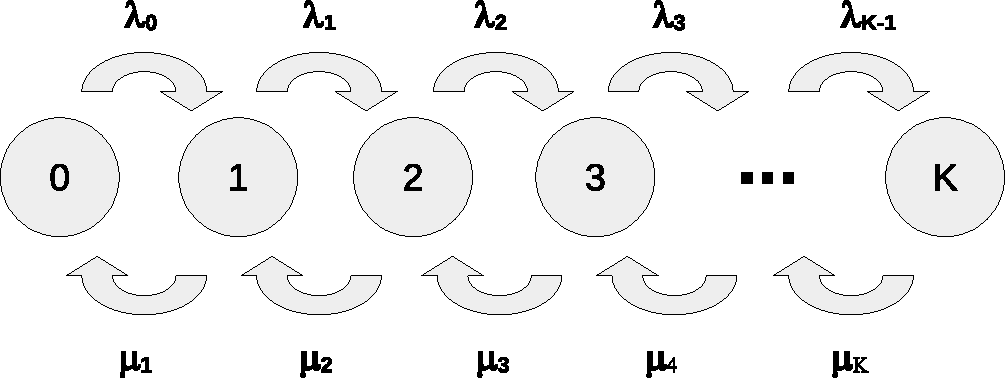
\includegraphics[width=0.6\textwidth]{ProofOfTheErlangCFormula-MarkovChain.pdf}
\end{center}
\caption{A birth-and-death process as a Markov chain}
\label{fig:BirthAndDEathProcess}
\end{figure}

\subsection{Arrival and service rate}

For the state-dependent arrival rate at the system in a service process with $K\in\mathbb{N}$ waiting and service places, the following applies to state $n\in\mathbb{N}_0$:

\begin{equation}\label{GleichungMarkovAnkunftsrate}
\lambda_n^{\rm Sys}:=\left\{\begin{matrix}
\lambda,&~n<K\;,\\
0,&~n=K\;,
\end{matrix}\right.
\end{equation}
where $\lambda>0$ is the arrival rate according to the customers. If there are already $n=K$ customers in the system, no further customers can enter the system, i.\,e., in this case, $\lambda^{\rm Sys}=0$.

The following applies to the state-dependent service rate for the entire system:
\begin{equation}\label{GleichungMarkovBedienrate}
\mu_n^{\rm Sys}:=\left\{\begin{matrix}
n\mu,&~n\le c\;,\\
c\mu,&~n>c\;,
\end{matrix}\right.
\end{equation}
where $\mu>0$ is the service rate of an individual operator.

\subsection{Transient state probabilities}

It is now assumed that the probability $p_n(t)$ that a total of $n\in\mathbb{N}_0$ customers are in the system at a given point in time $t\ge0$ is known. On this basis, the probability that $n\in\mathbb{N}_0$ customers are in the system at a time $t+\Delta t$ will be determined. Here, $\Delta t>0$ can be thought of as a small amount of time that has elapsed since time $t$. In the case of $n=0$, $p_0(t+\Delta t)$ is composed of the probability that there were already 0 people in the system at time $t$ and no customer arrived, and the probability that there was one customer in the system at time $t$ and that this customer was served within the time $\Delta t$. Furthermore, a customer could have arrived and already left the system again during the time period $\Delta t$, etc. However, compared to the first two probabilities mentioned, the probabilities for such combined events are negligible -- mathematically speaking, they converge to 0 faster than $\Delta t$ for $\Delta t\to0$. This is expressed by the Landau symbol $o(\Delta t)$. This results in $n=0$:
$$
p_0(t+\Delta t)=
p_0(t)(1-\Delta t\lambda_0^{\rm Sys})+p_1(t)\Delta t\mu_1^{\rm Sys}+o(\Delta t)\;.
$$
For $n=1,\ldots,K-1$, there is also the possibility that state $n$ was reached from state $n-1$:
$$
p_n(t+\Delta t)=
p_n(t)(1-\Delta t\lambda_n^{\rm Sys}-\Delta t\mu_n^{\rm Sys})+p_{n-1}(t)\Delta t\lambda_{n-1}^{\rm Sys}+p_{n+1}(t)\Delta t\mu_{n+1}^{\rm Sys}+o(\Delta t)\;.
$$
Finally, for $n=K$, the state can only be reached from the previous states $n$ and $n-1$:
$$
p_K(t+\Delta t)=
p_K(t)(1-\Delta t\mu_K^{\rm Sys})+p_{K-1}(t)\Delta t\lambda_{K-1}^{\rm Sys}+o(\Delta t)\;.
$$

\subsection{Stationary state probabilities}

Term transformation in the three equations above initially yields (for $n=1,\ldots,K-1$ in the middle equation):
\begin{eqnarray}
\frac{p_0(t+\Delta t)-p_0(t)}{\Delta t}&=&
-p_0(t)\lambda_0^{\rm Sys}+p_{1}(t)\mu_1^{\rm Sys}+\frac{o(\Delta t)}{\Delta t}\;,
\label{eq:StationaryStateProbabilities1}\\
\frac{p_n(t+\Delta t)-p_n(t)}{\Delta t}&=&
-p_n(t)(\lambda_n^{\rm Sys}+\mu_n^{\rm Sys})+p_{n+1}(t)\mu_{n+1}^{\rm Sys}+p_{n-1}(t)\lambda_{n-1}^{\rm Sys}+\frac{o(\Delta t)}{\Delta t}\;,
\nonumber\\
\frac{p_K(t+\Delta t)-p_K(t)}{\Delta t}&=&
-p_K(t)\mu_K^{\rm Sys}+p_{K-1}(t)\lambda_{K-1}^{\rm Sys}+\frac{o(\Delta t)}{\Delta t}\;.
\nonumber
\end{eqnarray}
If we now choose increasingly shorter time intervals for $\Delta t$, i.\,e., if we perform the limit transition $\Delta t\to0$, we obtain the following for $n=0,\ldots,K$ on the left-hand sides of the equations \eqref{eq:StationaryStateProbabilities1}:
$$
\lim_{\Delta t\to0}\frac{p_n(t+\Delta t)-p_n(t)}{\Delta t}=p'_n(t)\;.
$$
Furthermore, $\lim_{\Delta t\to0}\frac{o(\Delta t)} {\Delta t}=0$ applies according to the definition of $o(\Delta t)$. Thus, for $\Delta t\to0$, from \eqref{eq:StationaryStateProbabilities1}:
\begin{eqnarray}
p'_0(t)&=&
-p_0(t)\lambda_0^{\rm Sys}+p_{1}(t)\mu_1^{\rm Sys}\;,
\nonumber\\
p'_n(t)&=&
-p_n(t)(\lambda_n^{\rm Sys}+\mu_n^{\rm Sys})+p_{n+1}(t)\mu_{n+1}^{\rm Sys}+p_{n-1}(t)\lambda_{n-1}^{\rm Sys}\;,
\label{eq:StationaryStateProbabilities2}\\
p'_K(t)&=&
-p_K(t)\mu_K^{\rm Sys}+p_{K-1}(t)\lambda_{K-1}^{\rm Sys}\;.
\nonumber
\end{eqnarray}
Looking at a queueing system in steady state means looking at the system after a very long time, like for $t\to\infty$. The steady state is characterized in a system that reaches it, i.\,e., in which $\rho<1$, by the fact that the state probabilities stabilize, i.\,e., $p'_n(t)\to0$ applies for all $n=0,\ldots,K$ for $t\to\infty$. If we set $p'_n(t)=0$ in \eqref{eq:StationaryStateProbabilities2}, we obtain the following linear system of equations for the stationary, i.\,e., time-independent state probabilities $p_n:=\lim_{t\to\infty}p_n(t)$:
\begin{eqnarray}
p_1&=&
\frac{\lambda_0^{\rm Sys}}{\mu_1^{\rm Sys}}p_0\;,
\nonumber\\
p_{n+1}&=&
\frac{\lambda_n^{\rm Sys}}{\mu_{n+1}^{\rm Sys}}p_n+\frac{\mu_n^{\rm Sys}}{\mu_{n+1}^{\rm Sys}}p_n-\frac{\lambda_{n-1}^{\rm Sys}}{\mu_{n+1}^{\rm Sys}}p_{n-1}\;,
\label{eq:StationaryStateProbabilities3}\\
p_K&=&
\frac{\lambda_{K-1}^{\rm Sys}}{\mu_K^{\rm Sys}}p_{K-1}\;.
\nonumber
\end{eqnarray}

\begin{theorem}
With the above notations, the following applies:
\begin{equation}
p_n=\prod_{i=1}^n\frac{\lambda_{i-1}^{\rm Sys}}{\mu_i^{\rm Sys}}p_0 ~~~\textrm{für}~ n=1,\ldots,K
~~~\textrm{and}~~~
p_0=\left[\sum_{n=1}^K\prod_{i=1}^n\frac{\lambda_{i-1}^{\rm Sys}}{\mu_i^{\rm Sys}}+1\right]^{-1}\;.
\label{eq:StationaryStateProbabilities4}
\end{equation}
\end{theorem}

\begin{proof}
The proof for $p_n$, $n=1,\ldots,K$, is carried out by induction. The initial condition for induction follows directly from the first equation in \eqref{eq:StationaryStateProbabilities3}. Let us now assume that equation \eqref{eq:StationaryStateProbabilities4} holds for some $n\in\mathbb{N}$. Then, from the second equation of \eqref{eq:StationaryStateProbabilities3}, we obtain for $n+1$:
\begin{eqnarray*}
p_{n+1}&=&
\frac{\lambda_n^{\rm Sys}}{\mu_{n+1}^{\rm Sys}}p_n+\frac{\mu_n^{\rm Sys}}{\mu_{n+1}^{\rm Sys}}p_n-\frac{\lambda_{n-1}^{\rm Sys}}{\mu_{n+1}^{\rm Sys}}p_{n-1}\\&=&
\frac{\lambda_n^{\rm Sys}}{\mu_{n+1}^{\rm Sys}}\prod_{i=1}^n\frac{\lambda_{i-1}^{\rm Sys}}{\mu_i^{\rm Sys}}p_0+
\frac{\mu_n^{\rm Sys}}{\mu_{n+1}^{\rm Sys}}\prod_{i=1}^n\frac{\lambda_{i-1}^{\rm Sys}}{\mu_i^{\rm Sys}}p_0-
\frac{\lambda_{n-1}^{\rm Sys}}{\mu_{n+1}^{\rm Sys}}\prod_{i=1}^{n-1}\frac{\lambda_{i-1}^{\rm Sys}}{\mu_i^{\rm Sys}}p_0\\&=&
\prod_{i=1}^{n+1}\frac{\lambda_{i-1}^{\rm Sys}}{\mu_i^{\rm Sys}}p_0+
\underbrace{\left[\frac{\mu_n^{\rm Sys}\lambda_{n-1}^{\rm Sys}}{\mu_{n+1}^{\rm Sys}\mu_n^{\rm Sys}}-\frac{\lambda_{n-1}^{\rm Sys}}{\mu_{n+1}^{\rm Sys}}\right]}_{=0}
\prod_{i=1}^{n-1}\frac{\lambda_{i-1}^{\rm Sys}}{\mu_i^{\rm Sys}}p_0\;.
\end{eqnarray*}
The queueing system is always be in one of the states $0,\ldots,K$, i.\,e., the sum of all probabilities is 1 ($\sum_{n=0}^Kp_n=1$). Using the formula $p_n$, we obtain:
$$
p_0+\sum_{n=1}^K\prod_{i=1}^n\frac{\lambda_{i-1}^{\rm Sys}}{\mu_i^{\rm Sys}}p_0=1\;.
$$
Solving this equation for $p_0$ immediately yields the statement for $p_0$.
\end{proof}

\subsection{Stationary state probabilities for the actual arrival and service rates}

Previously, the formulas for the state probabilities used the arrival rate relative to the entire system $\lambda^{\rm Sys}$ and the service rate of the entire system $\mu^{\rm Sys}$. In the following, we will now use the arrival rates of the individual customers $\lambda$ and the service rates of the individual operators $\mu$. The variables $\lambda^{\rm Sys}$ and $\mu^{\rm Sys}$ are defined differently for three ranges: for $n=0$, for $n=1,\ldots,c$ and for $n=c+1,\ldots,K$. For this reason, $p_n$ is also calculated separately for these ranges in the following:

\subsubsection*{Calculation of $p_0$}

If we substitute the state probabilities from \eqref{GleichungMarkovAnkunftsrate} and \eqref{GleichungMarkovBedienrate} for $p_0$ in \eqref{eq:StationaryStateProbabilities4}, we
\begin{eqnarray*}
p_0&=&
\left[\sum_{n=1}^K\prod_{i=1}^n\frac{\lambda_{i-1}^{\rm Sys}}{\mu_i^{\rm Sys}}+1\right]^{-1} =
\left[\sum_{n=1}^K\left(
\lambda^n\cdot\frac{1}{\prod_{i=1}^{\min(n,c)}i\mu\cdot\prod_{i=\min(n,c)+1}^nc\mu}
\right)+1\right]^{-1}\\&=&
\left[\sum_{n=1}^c\frac{\lambda^n}{\mu^nn!}+\sum_{n=c+1}^K\frac{\lambda^n}{\mu^cc!\cdot(c\mu^{n-c})}+1\right]^{-1} =
\left[\sum_{n=1}^c\frac{\lambda^n}{\mu^nn!}+\sum_{n=c+1}^K\frac{\lambda^n}{\mu^nc!c^{n-c}}+1\right]^{-1}\;.
\end{eqnarray*}
With $a:=\frac{\lambda}{\mu}$ the following applies:
$$
p_0=
\left[\sum_{n=1}^c\frac{a^n}{n!}+\sum_{n=c+1}^K\frac{a^n}{c!c^{n-c}}+1\right]^{-1}\;.
$$
By choosing
\begin{equation}\label{MathematikErlangCn}
C_n:=\left\{\begin{array}{ll}
\displaystyle \frac{a^n}{n!}&~~\textrm{für}~n\le c\;,\\
\displaystyle \frac{a^n}{c!c^{n-c}}&~~\textrm{für}~c<n\le K
\end{array}\right.
\end{equation}
finally follows
$$
p_0=\left[\sum_{n=0}^KC_n\right]^{-1}\;.
$$

\subsubsection*{Calculation of $p_n$ for $n=1,\ldots,c$}

If we substitute the state probabilities from \eqref{GleichungMarkovAnkunftsrate} and \eqref{GleichungMarkovBedienrate} for $p_n$ in \eqref{eq:StationaryStateProbabilities4}, we obtain the following with the definition of $C_n$ in \eqref{MathematikErlangCn} for $n=1,\ ...c$:
$$
p_n=
\prod_{i=1}^n\frac{\lambda_{i-1}^{\rm Sys}}{\mu_i^{\rm Sys}}\cdot p_0=
\prod_{i=1}^n\frac{\lambda}{n\mu}\cdot p_0=
\frac{a^n}{n!}\cdot p_0=
C_np_0\;.
$$

\subsubsection*{Calculation of $p_n$ for $n=c+1,\ldots,K$}

If we substitute the state probabilities from \eqref{GleichungMarkovAnkunftsrate} and \eqref{GleichungMarkovBedienrate} for $p_n$ in \eqref{eq:StationaryStateProbabilities4}, we obtain the following with the definition of $C_n$ in \eqref{MathematikErlangCn} für $n=c+1,\ldots,K$:
\begin{eqnarray*}
p_n&=&
\prod_{i=1}^n\frac{\lambda_{i-1}^{\rm Sys}}{\mu_i^{\rm Sys}}\cdot p_0=
\prod_{i=1}^c\frac{\lambda}{n\mu}\cdot\prod_{i=c+1}^n\frac{\lambda}{c\mu}\cdot p_0=
\frac{a^n}{c!c^{n-c}}\cdot p_0=
C_np_0\;.
\end{eqnarray*}

The above considerations for $p_n$ can be summarized in the following theorem:

\begin{theorem}
With the choice of $C_n$ according to \eqref{MathematikErlangCn}, the following applies to the state probabilities $p_n$ in a birth and death process with arrival and service rates according to \eqref{GleichungMarkovAnkunftsrate} and \eqref{GleichungMarkovBedienrate}:
\begin{equation}\label{MathematikPn}
p_n=\left\{\begin{array}{ll}
\displaystyle \left[\sum_{i=0}^KC_i\right]^{-1}&~~\textrm{für}~n=0\;,\\
\displaystyle C_n p_0&~~\textrm{für}~n>0\;.
\end{array}\right.
\end{equation}
\end{theorem}



\section{The Erlang C formula}\label{Result}

With the choice of $K:=\infty$, the following initially applies to $C_n$ (see formula \eqref{MathematikErlangCn}):
\begin{equation*}
C_n:=\left\{\begin{array}{ll}
\displaystyle \frac{a^n}{n!}&~~\textrm{für}~n<c\;,\\
\displaystyle \frac{a^n}{c!c^{n-c}}&~~\textrm{für}~n\ge c\;.
\end{array}\right.
\end{equation*}
The probability that there are no customers in the system, $p_0$, is calculated in this case by
$$
1=
p_0+\sum_{n=1}^\infty C_np_0=
p_0\left(1+\sum_{n=1}^\infty C_n\right)
$$
to:
\begin{eqnarray*}
p_0&=&
\left[1+\sum_{n=1}^\infty C_n\right]^{-1}=
\left[\sum_{n=0}^{c-1}\frac{a^n}{n!}+\sum_{n=c}^\infty\frac{a^n}{c!c^{n-c}}\right]^{-1}=
\left[\sum_{n=0}^{c-1}\frac{a^n}{n!}+\frac{a^c}{c!}\sum_{n=0}^\infty\frac{a^n}{c^n}\right]^{-1}\\&=&
\left[\sum_{n=0}^{c-1}\frac{a^n}{n!}+\frac{a^c}{c!}\cdot\frac{1}{1-\frac{a}{c}}\right]^{-1}=
\left[\sum_{n=0}^{c-1}\frac{a^n}{n!}+\frac{a^c\cdot c}{c!(c-a)}\right]^{-1}\;.
\end{eqnarray*}
In the calculation
$$
\sum_{n=0}^\infty\left(\frac{a}{c}\right)^n=\frac{1}{1-\frac{a}{c}}
$$
In the penultimate calculation step, the geometric series was used and the assumption was made that in the case of a queueing model without cancelations, $\lambda<c\mu$ must apply, i.\,e., $\frac{a}{c}<1$ must be true, which is necessary for the convergence of the series.

On this basis, the waiting time distribution $P(W\le t)$ can now be determined for an Erlang C model:
{
\allowdisplaybreaks
\begin{eqnarray*}
P(W\le t)&=&
\sum_{n=0}^{c-1}C_np_0+\sum_{n=c}^\infty F_{c\mu,n-c+1}(t)C_np_0\\&=&
\sum_{n=0}^{c-1}C_np_0+\sum_{n=c}^\infty \int_0^t \frac{(c\mu)^{n-c+1}x^{n-c}}{(n-c)!}\mathrm{e}^{-c\mu x}\,\mbox{d}x C_np_0\\&=&
\sum_{n=0}^{c-1}C_np_0+\int_0^t\sum_{n=c}^\infty \frac{(c\mu)^{n-c+1}x^{n-c}}{(n-c)!}\mathrm{e}^{-c\mu x}\,\mbox{d}x C_np_0\\&=&
% \sum_{n=0}^{c-1}C_np_0+p_0c\mu\int_0^t \mathrm{e}^{-c\mu x}\sum_{n=0}^\infty \frac{(c\mu x)^n}{n!}\cdot\frac{a^{n+c}}{c!c^n}\,\mbox{d}x\\&=&
\sum_{n=0}^{c-1}C_np_0+p_0\frac{a^cc\mu}{c!}\int_0^t \mathrm{e}^{-c\mu x}\sum_{n=0}^\infty \frac{(\mu xa)^n}{n!}\,\mbox{d}x\\&=&
\sum_{n=0}^{c-1}C_np_0+p_0\frac{a^cc\mu}{c!}\int_0^t \mathrm{e}^{-c\mu x}\cdot \mathrm{e}^{a\mu x}\,\mbox{d}x\\&=&
\sum_{n=0}^{c-1}C_np_0+p_0\frac{a^cc\mu}{c!}\left[-\frac{1}{(c-a)\mu}\mathrm{e}^{-(c-a)\mu x}\right]_{x=0}^{x=t}\\&=&
\sum_{n=0}^{c-1}C_np_0-p_0\frac{a^cc}{c!(c-a)}\left(\mathrm{e}^{-(c-a)\mu t}-1\right)\\&=&
% p_0\underbrace{\left(\sum_{n=0}^{c-1}\frac{a^n}{n!}+\frac{a^c\cdot c}{c!(c-a)}\right)}_{=p_0^{-1}}-p_0\frac{a^cc}{c!(c-a)}\mathrm{e}^{-(c-a)\mu t}\\&=&
1-p_0\frac{a^cc}{c!(c-a)}\mathrm{e}^{-(c-a)\mu t}\;.
\end{eqnarray*}
}
Using the definition
\begin{tcolorbox}
\begin{equation}\label{MMcP1ErlangCBeweis}
P_1:=p_0\frac{a^cc}{c!(c-a)}=\frac{\frac{a^cc}{c!(c-a)}}{\sum_{n=0}^{c-1}\frac{a^n}{n!}+\frac{a^c\cdot c}{c!(c-a)}}
\end{equation}
\end{tcolorbox}
this ultimately yields the usual Erlang C formula:
\begin{tcolorbox}
$$
P(W\le t)=1-P_1\mathrm{e}^{-(c-a)\mu t}\;.
$$
\end{tcolorbox}

\subsection{Characteristics}

In the case of an M/M/c system, the other characteristics can be derived directly from the already determined values $p_n$ and $C_n$:
\begin{itemize}
\item
\emph{Average queue length:}~\\
Using the definition of $P_1$ from \eqref{MMcP1ErlangCBeweis}, the following initially applies for $n>c$:
$$
p_n=C_np_0=\frac{a^n}{c!c^{n-c}}p_0=P_1\rho^{n-c}(1-\rho)\,.
$$
This immediately gives us the average queue length with the definition of the expected value:
\begin{eqnarray*}
\mathbf{E}[N_Q]&=&
\sum_{n=c+1}^\infty(n-c)p_n=
P_1(1-\rho)\sum_{n=c+1}^\infty(n-c)\rho^{n-c}\\&=&
P_1(1-\rho)\sum_{n=1}^\infty n\rho^n=
P_1(1-\rho)\sum_{n=0}^\infty n\rho^n=
P_1(1-\rho)\rho\sum_{n=1}^\infty n\rho^{n-1}\;.
\end{eqnarray*}
Since $f'(\rho)=n\rho^{n-1}$ holds for $f(\rho):=\rho^n$, the following also applies:
$$
\mathbf{E}[N_Q]=P_1(1-\rho)\rho\sum_{n=1}^\infty \left[\rho^n\right]'\,.
$$
Due to the absolute convergence of the series caused by the fact that $\rho<1$, limit process and differentiation can be interchanged. Applying the geometric series ($\sum_{n=0}^\infty a^n=\frac{1}{1-a}$ for $|a|<1$), the following applies:
\begin{eqnarray*}
\mathbf{E}[N_Q]&=&
P_1(1-\rho)\rho\left[\sum_{n=1}^\infty \rho^n\right]'=
P_1(1-\rho)\rho\left[\frac{1}{1-\rho}\right]'=
P_1(1-\rho)\rho\frac{0-(-1)}{(1-\rho)^2}\\&=&
P_1\frac{\rho}{1-\rho}=
P_1\frac{a}{c-a}\;.
\end{eqnarray*}
\item
\emph{Average number of customers in the system:}~\\
The average number of customers in the system is calculated as the sum of the average queue length $\mathbf{E}[N_Q]$ and the average number of customers being served $a$:
$$
\mathbf{E}[N]=P_1\frac{a}{c-a}+a\;.
$$
The fact that the workload $a$ corresponds precisely to the average number of customers being served is a consequence of Little's law.
\item
\emph{Average waiting time:}~\\
Using Little's law, the mean waiting time can be directly calculated from $\mathbf{E}[N_Q]$:
$$
\mathbf{E}[W]=
\frac{1}{\lambda}\mathbf{E}[N_Q]=
P_1\frac{1}{\lambda}\frac{a}{c-a}=
P_1\frac{\frac{1}{\mu}}{c-a}=
P_1\frac{1}{c\mu-\lambda}\;.
$$
\item
\emph{Average residence time:}~\\
The average residence time is composed of the average waiting time $\mathbf{E}[W]$ and the average service time $\mathbf{E}[S]=\frac{1}{\mu}$:
$$
\mathbf{E}[V]=P_1\frac{1}{c\mu-\lambda}+\frac{1}{\mu}\;.
$$
\end{itemize}

In summary:
\begin{tcolorbox}
\begin{eqnarray*}
\mathbf{E}[N_Q]&=&P_1\frac{a}{c-a}\;,\\
\mathbf{E}[N]&=&P_1\frac{a}{c-a}+a\;,\\
\mathbf{E}[W]&=&P_1\frac{1}{c\mu-\lambda}\;,\\
\mathbf{E}[V]&=&P_1\frac{1}{c\mu-\lambda}+\frac{1}{\mu}\;.
\end{eqnarray*}
\end{tcolorbox}

\end{document}
